\documentclass{tufte-handout}
\usepackage{graphicx}
\graphicspath{ {./images/} }
\title{Introduction to Neural Networks}

\begin{document}
\maketitle
\begin{abstract}
Neural Networks try to resemble the way humans make decisions and the 
way neurons in the human brain take in data and act on input.
\end{abstract}

\section{Introduction}
A neuron usually has a couple parts to it. There are the \textbf{dendrites}, which are in charge of
	receiving incoming signals from other neurons. 
The signals then travel through the cell body and the \textbf{axons} all the way to the connections at the 
	end of the axons.
These neurons are all connected to many other neurons each, so any attempt to model these connections will
	necessarily use up a lot of connections.

In computer science, we hae something resembling a neuron, except that the way we model decisions is a bit 
	different. 

\begin{marginfigure}
	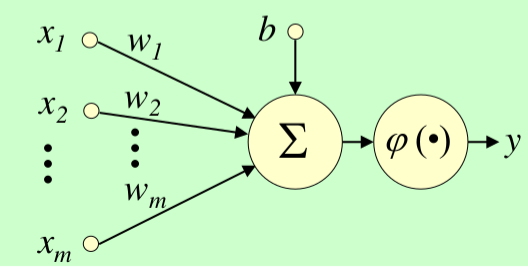
\includegraphics[scale=0.3]{nn_diagram}
	\caption{We take a set of inputs $x_{1}\dots x_{n}$ and pass each of these through a corresponding 
		\textbf{weight function} $w_{1}\dots w_{n}$. In the actual node body, we take the sum of the weight
		functions connecting the current neuron to the ones in the previous layer. This sum $\Sigma$ is then 
		passed through the final \textbf{activation function} $\varphi$, which gives the final output for this
		neuron.}
\end{marginfigure}

Neural networks are usually represented by a connected graph of neurons, usually organized in layers. 
There are a couple types:
\begin{enumerate}
	\item \textbf{Feedforward}: In these types, the signals only flow in one direction.
	\item \textbf{Recurrent}: In recurrent neural networks, there is feed forward functionality, but 
			there can also be feedback to the neurons.
\end{enumerate}

In a neural network, we would usually have $k$ output layers, which might represent the confidence with which 
	we classify or predict a certain value for our model.
Let the final value of our model ve $y(x)$ for some input vector $x$. The error value for a neural network
	would then be
\[ e = d- y\]

	which we of course want to minimize.

\subsection{Perceptron Algorithm}
The perceptron algorithm is an algorithm which can learn the classification from the data. 
How does it do this?
It only updates the set of weights when it makes a mistake in classifying or regressing(?) the testing data.

Originally, with a single neuron, the algorithm could only handle the cases that were 
\textbf{linearly separable}. 
For example, training a model to learn the behavior of the XOR function is not possible with 
	only a single neuron, again since the training data is not linearly separable.
However, with a simple two-layer network we can easily model the behavior of XOR.

So, for a single neuron, updating the values of $\mathbf{w}$  is quite easy, since we only have a single value
	to update once we have estimated the model. 
How do we do this when we have multiple values in $\mathbf{w}$? 
We have to use \textbf{Back-Propagation}.

\textbf{Back-Propagation} tries to maximize the values starting at the output nodes. 
The error value then moves back through the layers, and we calculate the error for the individual neurons 
	in a backward fashion.
An iteration in which all the testing samples are seen at least once is called an \textbf{epoch}.

Once we do the back-propagation, how do we know when to stop?
We can have several criteria:
\begin{enumerate}
		\item Stop when the cost function is lower than a trheshold (when it's ``good enough")
		\item Also can stop when the gradient is lower than a certain function.
		\item When the \textbf{learning curve} over several iterations remains stable.
\end{enumerate}

Remember the \textbf{activation function} tells us how confident we are in our prediction, and it lies 
	between 0 and 1, for not confident and confident, respectively.
What functions can map the entire number interval into 0 and 1? 
The old standard was the \textbf{sigmoidal function}, which is
\[ f(v) = \frac{1}{1 + e^{-av}}\]
There appears to be some issues with this function. 
Although it is \textbf{continuously differentiable}, the gradients apparently go to infinity pretty quickly?
This function used to be the standard, but not so much anymore.

Now, the standard for activation functions has become \textbf{REctified Linear Units (RELU)}. 
This function takes the form
\[ f(v) = tanh(\alpha v)\]

Both of these functions are \textbf{non-linear}.

Another question remains: What should our learning rate be?
We could either choose to make it larger or smaller, and there are consequences for both.
If we make it smaller, then the algorithm will take slower, since to find the global maximum it 
	will have to be adjusted several times. However, the learning rate $\varphi$ will proceed along
	a smoother trajectory to the final learning rate.

For a larger $\varphi$,  the effects are the opposite: there is a faster training cycle but more
	oscillation from the different epochs.

\begin{marginfigure}
		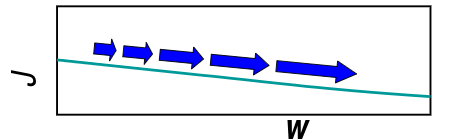
\includegraphics[scale=0.4]{momentum}
		\caption{ The \textbf{momentum} is a technique for speeding up the training. When multiple
			gradients lie in the same direction, we increase them with a multiplier. The update 
			to the learning rate is smaller when the gradients are in different directions.}
\end{marginfigure}

Historically, neural networks only used one layer due to computational constraints.
However, in the recent years \textbf{Deep Neural Networks} have become more popular. 
These networks merel contain more than one hidden layer.
\end{document}
